% document formatting
\documentclass[10pt]{article}
\usepackage[utf8]{inputenc}
\usepackage[left=1in,right=1in,top=1in,bottom=1in]{geometry}
\usepackage[T1]{fontenc}
\usepackage{xcolor}

% math symbols, etc.
\usepackage{amsmath, amsfonts, amssymb, amsthm}

% lists
\usepackage{enumerate}

% images
\usepackage{graphicx} % for images

% code blocks
\usepackage{minted, listings} 

% verbatim greek
\usepackage{alphabeta}

\graphicspath{{./assets/images}}

\newcommand{\solution}{\textbf{Solution:}} 
\newcommand{\example}{\textbf{Example: }}

\title{EC ENGR 102 Week 5}

\author{Aidan Jan}
\date{\today}

\begin{document}
\maketitle

\subsection*{Sawtooth Signal}
The sawtooth signal is given by $f(t) = t \mod 1$.  It is plotted below:
\begin{center}
    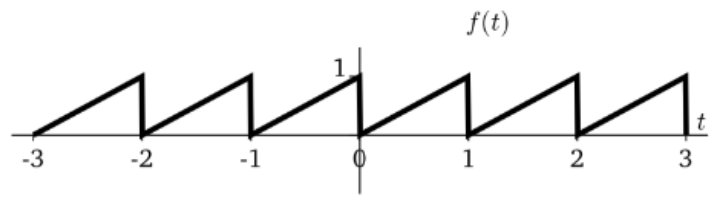
\includegraphics[scale=0.9]{W4_13.png}
\end{center}
This signal has a period of $T_0 = 1$.  Now, when $k = 0$,
\begin{align*}
    c_0 &= \int_0^1 te^0 \text{d}t\\
    &= \left.\frac{t^2}{2}\right|_0^1\\
    &= \frac{1}{2}
\end{align*}
This is also the Fourier series of the time-limited signal $f(t) = t$ on the interval $[0, 1)$.  The time-limited signal can be made periodic via a periodic extension.

\subsection*{Fourier Series Properties}
There are interesting symmetries and properties of the Fourier series that are worth expanding upon.
\begin{itemize}
    \item $c_0$ \textbf{is the average of the signal}.  Not that for $k = 0$, we have that
    \[c_0 = \frac{1}{T_0} \int_{t_0}^{t_0 + T_0} f(t) \text{d}t\]
    Thus, $c_0$ is exactly the time-averaged mean of the signal and corresponds to a constant value (i.e., it has no sinusoidal component).  For this reason, it is sometimes called the "DC component."  DC stands for direct current in circuits, and refers to non-alternating (sinusoidal) currents.  The DC component is the average value taken on by a signal.
\end{itemize}

\subsection*{Fourier Symmetry}
We can apply Euler's formula to re-write the Fourier coefficients, and reveal some symmetries:
\begin{align*}
    c_k &= \frac{1}{T_0} \int_{t_0}^{t_0 + T_0} f(t) e^{-j\frac{2\pi kt}{T_0}}\text{d}t\\
    &= \frac{1}{T_0} \int_{t_0}^{t_0 + T_0} f(t) \left[\cos\left(\frac{2\pi k}{T_0}t\right) - j \sin\left(\frac{2\pi k}{T_0}t\right)\right]\text{d}t
    &= \frac{1}{T_0} \int_{t_0}^{t_0 + T_0} f(t) \cos\left(\frac{2\pi k}{T_0}t\right) \text{d}t - \frac{j}{T_0} \int_{t_0}^{t_0 + T_0} f(t) \sin\left(\frac{2\pi k}{T_0}t\right)\text{d}t
\end{align*}
In the above equation, the left term is the real part, the right term is the imaginary part.\\\\
If $f(t)$ is real, then so are:
\begin{align*}
    \mathfrak{R}(c_k) &= \frac{1}{T_0}\int_{t_0}^{t_0 + T_0}f(t)\cos\left(\frac{2\pi k}{T_0}t\right)\text{d}t\\
    \mathfrak{I}(c_k) &= -\frac{1}{T_0}\int_{t_0}^{t_0 + T_0}f(t)\sin\left(\frac{2\pi k}{T_0}t\right)\text{d}t
\end{align*}
Therefore, for $f(t)$ real, and using the fact that $\cos(k)$ is even and $\sin(k)$ is odd, we have the following symmetries:
\begin{align}
    \mathfrak{R}(c_k) &= \mathfrak{R}(c_{-k})\\
    \mathfrak{I}(c_k) &= \mathfrak{I}(c_{-k})\\
    c_k^* &= c_{-k}\\
    |c_k| &= |c_{-k}|\\
    \angle c_k &= -\angle c_k^*\\
    c_k &= c_{-k}\hspace{1cm} \text{(only if $x(t)$ is even)}\\
    c_k &= -c_{-k}\hspace{1cm} \text{(only if $x(t)$ is odd)}
\end{align}
\subsubsection*{Proof of (1)}
\begin{align*}
    \mathfrak{R}(c_{-k}) &= \frac{1}{T_0} \int_{t_0}^{t_0 + T_0}f(t) \cdot \cos\left(-\frac{2\pi k}{T_0} t\right) \text{d}t\\
    &= \frac{1}{T_0} \int_{t_0}^{t_0 + T_0}f(t) \cdot \cos\left(\frac{2\pi k}{T_0} t\right) \text{d}t\\
    &= \mathfrak{R}(c_{-k})
\end{align*}
\subsubsection*{Proof of (2)}
\begin{align*}
    \mathfrak{I}(c_{-k}) &= -\frac{1}{T_0} \int_{t_0}^{t_0 + T_0}f(t) \cdot \sin\left(-\frac{2\pi k}{T_0} t\right) \text{d}t\\
    &= \frac{1}{T_0} \int_{t_0}^{t_0 + T_0}f(t) \cdot \sin\left(\frac{2\pi k}{T_0} t\right) \text{d}t\\
    &= \mathfrak{I}(c_{-k})
\end{align*}
\subsubsection*{Proof of (3)}
\begin{align*}
    c_k &= \mathfrak{R}(c_k) + j \cdot \mathfrak{I}(c_k)\\
    c_k^* &- \mathfrak{R}(c_k) - j \cdot \mathfrak{I}(c_k)\\
    &= \mathfrak{R}(c_-k) + j \cdot \mathfrak{I}(c_-k)\\
    &= c_{-k}
\end{align*}
\subsubsection*{Proof of (4)}
\begin{align*}
    |c_k| &= \sqrt{\mathfrak{R}^2(c_k) + \mathfrak{I}^2(c_k)}\\
    |c_{-k}| &= \sqrt{\mathfrak{R}^2(c_k) + \mathfrak{I}^2(c_{-k})}\\
    &= \sqrt{\mathfrak{R}^2(c_k) + (-\mathfrak{I}(c_k))^2}\\
    &= |c_k|
\end{align*}
\subsubsection*{Proof of (5)}
\begin{align*}
    \angle c_k &= \arctan \left(\frac{\mathfrak{R}(c_k)}{\mathfrak{I}(c_k)}\right)\\
    &= \arctan \left(\frac{\mathfrak{R}(c_{-k})}{\mathfrak{I}(c_{-k})}\right)\\
    &= \arctan \left(\frac{\mathfrak{R}(c_{k})}{-\mathfrak{I}(c_k)}\right)\\
    &= \angle c_{-k}
\end{align*}
\subsubsection*{Proof of (6)}
\begin{align*}
    c_k &= \frac{1}{T_0} \int_{0}^{T_0} x(t) e^{-jk\omega_0 t} \text{d}t\\
    c_{-k} &= \frac{1}{T_0} \int_{0}^{T_0} x(t) e^{jk\omega_0 t}\text{d}t\\
    \intertext{Let $u = -t$.}
    &= -\frac{1}{T_0} \int_{0}^{-T_0} x(-u) \cdot e^{-jk\omega_0 u} \text{d}u\\
    &= \frac{1}{T_0} \int_{-T_0}^0 x(u) \cdot e^{-jk\omega_0 u} \text{d}u\\
    &= c_k
\end{align*}
\subsection*{Fourier Series Properties}
\begin{itemize}
    \item If $x(t)$ is even, then $x(t) = x(-t)$, and therefore, $c_k = c_{-k}$.  You can see this by realizing that $kt$ only appears in the complex exponential, and therefore negating $t$ has the same effect as negating $k$.
    \[x(t) \text{ even} \Longrightarrow c_k = c_{-k}\]
    \item If $x(t)$ is odd, then $x(t) = -x(-t)$, and therefore, $c_k = -c_{-k}$.  This holds for the same reason as for the even case.
    \[x(t) \text{ odd} \Longrightarrow c_k = -c_{-k}\]
    \item Combining facts, we have that if $x(t)$ is even and real, then $c_k = c_{-k}$ and $c_{-k} = c_k^*$, and so $c_k = c_k^*$.  This means that $c_k$ must be real.
    \[x(t) \text{ even and real} \Longrightarrow c_k \text{ real}\]
    \item If $x(t)$ is odd and real, then $c_k = -c_{-k}$, and because $c_{-k} = c_k^*$, then $c_k = -c_k^*$.  This means that $c_k$ must be imaginary.
    \[x(t) \text{ odd and real} \Longrightarrow c_k \text{ imaginary}\]
\end{itemize}

\subsection*{Perseval's Theorem}
Suppose we want to find the power of a complex signal:
\[\frac{1}{T_0} \int_{t_0}^{t_0 + T_0} |x(t)|^2 \text{ d}t\]
Since $x(t)$ is complex, we split the square to $x(t) \cdot x(t)^*$.  Therefore,
\begin{align*}
    &= \frac{1}{T_0} \int_{t_0}^{t_0 + T_0} x(t) x(t)^* \text{d}t\\
    &= \frac{1}{T_0} \int_{t_0}^{t_0 + T_0} \left[\sum_{k=-\infty}^\infty c_k e^{jk\omega_0 t}\right] \left[\sum_{n=-\infty}^\infty c_n^* e^{-jn\omega_0 t}\right] \text{d}t
    \intertext{We can then switch the order of the summation and integral.}
    &= \frac{1}{T_0} \sum_{k = -\infty}^\infty c_k \sum_{k = -\infty}^\infty c_n^* \cdot \int_{t_0}^{t_0 + T_0} e^{j(k-n)\omega_0 t} \text{d}t\\
    \intertext{Notice that the integral returns $0$ when $k \neq n$, and $T_0$ when $k = n$.  This is because if you expand the exponential using Euler's formula, then you are integrating a cosine and sin over one period, the periods of which will cancel out.  Therefore,}
    &= \frac{1}{T_0} \sum_{-\infty}^\infty c_k \cdot c_k^* \cdot T_0\\
    &= \sum_{k=-\infty}^\infty |c_k|^2
\end{align*}

\textbf{Everything before this point is fair game on Midterm 1.}\\

\section*{Aperiodic Signals}
\begin{itemize}
    \item The Fourier series can model (almost) any \textbf{periodic} or \textbf{time-limited} function as a sum of complex exponentials.  However, most signals we encounter are not necessarily periodic or time-limited.
    \item The \textbf{Fourier transform} allows us to calculate the spectrum of aperiodic signals.
\end{itemize}

\subsection*{Intuition of going from Fourier series to Fourier transform}
Extending Fourier series to the Fourier transform is fairly intuitive.\\\\
The idea is the following:
\begin{itemize}
    \item We can calculate the Fourier series of a periodic or time-limited signal, over some interval of length $T_0$.
    \item A signal that is not periodic can be viewed as a periodic signal, where $T_0$ is infinite.  As $T_0$ is infinite, it never repeats.
    \item But the point is that we can replace our Fourier series calculation as, instead of being over a finite period, $T_0$, being over all time, from $t = -\infty$ to $\infty$.
    \item Mathematically, we can calculate the Fourier series of $f(t)$ over the interval $[-T/2. T/2)$ via:
    \[f(t) = \sum_{k = -\infty}^\infty c_k e^{jk\omega_0 t}\]
    with 
    \[c_k = \frac{1}{T} \int_{-T/2}^{T/2} f(t) e^{-jk\omega-0}\text{d}t\]
    where $\omega_0 = 2\pi/T$.  In the Fourier transform, we're now going to let $T \rightarrow \infty$.
\end{itemize}
\example\\
\begin{center}
    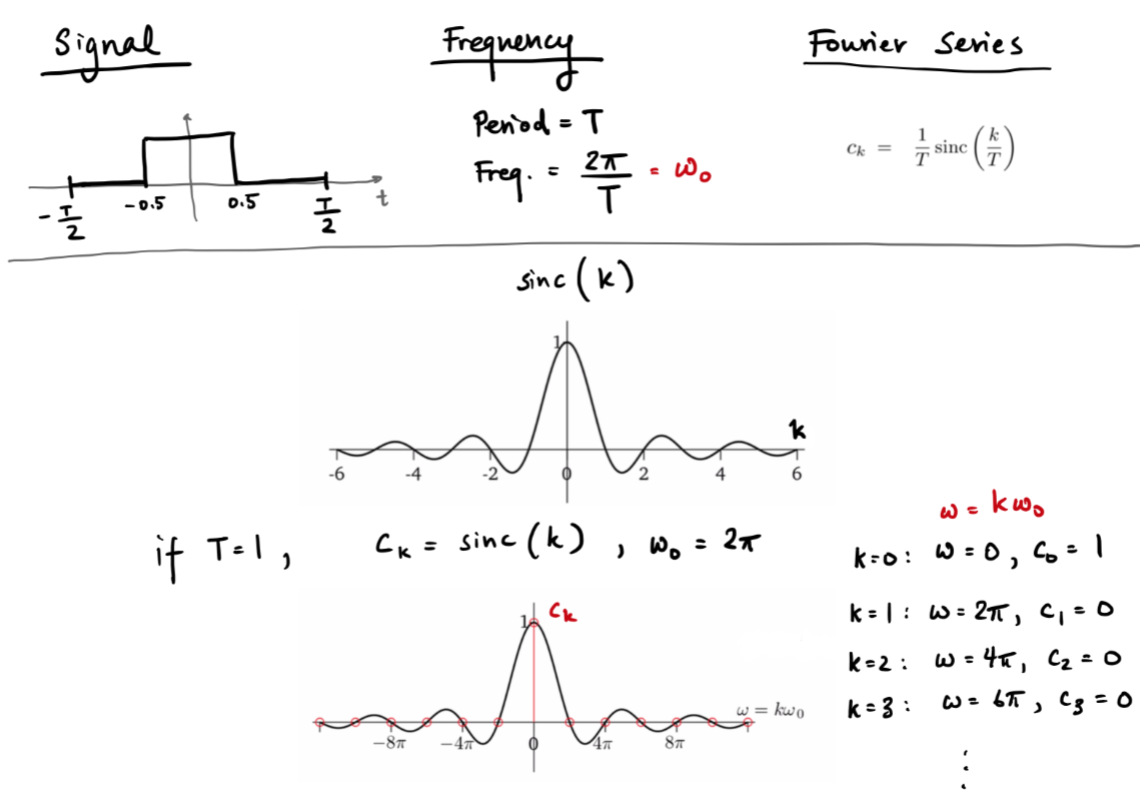
\includegraphics[scale=0.65]{W5_1.png}
\end{center}


\end{document}